\subsection{Space Partitioning}

A naive implementation of non-bonded forces would test every possible pair of particles, for a total of $n(n-1)/2$ possibilities, with $n$ the number of interacting particles (for our coarse grained DNA model, $n$ would be the number of sites, which is three times the number of monomers).
However, most of these considered pairs are superfluous because the particles are separated too far apart and their interaction is negligible. This $O\left(\frac{n(n-1)}{2}\right) = O(n^2)$ complexity is undesirable for performance reasons.
A known technique to improve this algorithmic complexity is called \emph{spatial partitioning}. An explanation (and application to multiprocessor scaling) can, for instance, be found in \cite{plimpton1995fast}.

By splitting the world into smaller partitions, or \emph{boxes}, one only has to check for interactions between particles in nearby partitions.
In the ideal case, if the number of interacting particles contained per box is a constant $x$, the amount of boxes becomes $n/x$. Interactions need only be checked between particles in the same box for $x(x-1)/2$ pairs, and between particles in a given box and particles in the adjacent boxes. If each box has $z$ neighbouring boxes, then there are $zx^2/2$ such pairs. The total complexity of this problem thus reduces to 
$O\left(
	\left[ \frac{x(x-1)}{2} + \frac{zx^2}{2} \right]
		\cdot \frac{n}{x}
\right) = O(n)$,
linear in the number of interacting particles.

It is easy to show that we cannot do any better than $O(n)$ via this partitioning trick, and that choosing the number of boxes $b$ to be proportional to $n$ is the ideal case.
Indeed, assume that we would instead take the number of boxes $b \sim n^\alpha$. Then the average number of particles per box $x$ would be proportional to $n^{1 - \alpha}$. Using the reasoning above, we find that the average number of interaction pairs that would be considered is proportional to $x^2 b = n^{2(1 - \alpha)} n^\alpha = n^{2 -\alpha}$. It seems that we can make the algorithmic complexity sub-linear by choosing $\alpha > 1$, however, we also have to iterate over all the boxes, and their number is proportional to $n^\alpha$. In other words, the total algorithmic time complexity is $O(n^{2 - \alpha} + n^\alpha)$, with the optimal value of $\alpha$ equal to one.


\begin{figure}[htb]
       \begin{center}
               \scalebox{0.9}{
                        \nonstopmode
                        % GNUPLOT: LaTeX picture with Postscript
\begingroup
  \makeatletter
  \providecommand\color[2][]{%
    \GenericError{(gnuplot) \space\space\space\@spaces}{%
      Package color not loaded in conjunction with
      terminal option `colourtext'%
    }{See the gnuplot documentation for explanation.%
    }{Either use 'blacktext' in gnuplot or load the package
      color.sty in LaTeX.}%
    \renewcommand\color[2][]{}%
  }%
  \providecommand\includegraphics[2][]{%
    \GenericError{(gnuplot) \space\space\space\@spaces}{%
      Package graphicx or graphics not loaded%
    }{See the gnuplot documentation for explanation.%
    }{The gnuplot epslatex terminal needs graphicx.sty or graphics.sty.}%
    \renewcommand\includegraphics[2][]{}%
  }%
  \providecommand\rotatebox[2]{#2}%
  \@ifundefined{ifGPcolor}{%
    \newif\ifGPcolor
    \GPcolortrue
  }{}%
  \@ifundefined{ifGPblacktext}{%
    \newif\ifGPblacktext
    \GPblacktexttrue
  }{}%
  % define a \g@addto@macro without @ in the name:
  \let\gplgaddtomacro\g@addto@macro
  % define empty templates for all commands taking text:
  \gdef\gplbacktext{}%
  \gdef\gplfronttext{}%
  \makeatother
  \ifGPblacktext
    % no textcolor at all
    \def\colorrgb#1{}%
    \def\colorgray#1{}%
  \else
    % gray or color?
    \ifGPcolor
      \def\colorrgb#1{\color[rgb]{#1}}%
      \def\colorgray#1{\color[gray]{#1}}%
      \expandafter\def\csname LTw\endcsname{\color{white}}%
      \expandafter\def\csname LTb\endcsname{\color{black}}%
      \expandafter\def\csname LTa\endcsname{\color{black}}%
      \expandafter\def\csname LT0\endcsname{\color[rgb]{1,0,0}}%
      \expandafter\def\csname LT1\endcsname{\color[rgb]{0,1,0}}%
      \expandafter\def\csname LT2\endcsname{\color[rgb]{0,0,1}}%
      \expandafter\def\csname LT3\endcsname{\color[rgb]{1,0,1}}%
      \expandafter\def\csname LT4\endcsname{\color[rgb]{0,1,1}}%
      \expandafter\def\csname LT5\endcsname{\color[rgb]{1,1,0}}%
      \expandafter\def\csname LT6\endcsname{\color[rgb]{0,0,0}}%
      \expandafter\def\csname LT7\endcsname{\color[rgb]{1,0.3,0}}%
      \expandafter\def\csname LT8\endcsname{\color[rgb]{0.5,0.5,0.5}}%
    \else
      % gray
      \def\colorrgb#1{\color{black}}%
      \def\colorgray#1{\color[gray]{#1}}%
      \expandafter\def\csname LTw\endcsname{\color{white}}%
      \expandafter\def\csname LTb\endcsname{\color{black}}%
      \expandafter\def\csname LTa\endcsname{\color{black}}%
      \expandafter\def\csname LT0\endcsname{\color{black}}%
      \expandafter\def\csname LT1\endcsname{\color{black}}%
      \expandafter\def\csname LT2\endcsname{\color{black}}%
      \expandafter\def\csname LT3\endcsname{\color{black}}%
      \expandafter\def\csname LT4\endcsname{\color{black}}%
      \expandafter\def\csname LT5\endcsname{\color{black}}%
      \expandafter\def\csname LT6\endcsname{\color{black}}%
      \expandafter\def\csname LT7\endcsname{\color{black}}%
      \expandafter\def\csname LT8\endcsname{\color{black}}%
    \fi
  \fi
  \setlength{\unitlength}{0.0500bp}%
  \begin{picture}(7680.00,7680.00)%
    \gplgaddtomacro\gplbacktext{%
      \colorrgb{0.00,0.00,0.00}%
      \put(866,845){\makebox(0,0)[r]{\strut{}0}}%
      \colorrgb{0.00,0.00,0.00}%
      \put(866,1627){\makebox(0,0)[r]{\strut{}500}}%
      \colorrgb{0.00,0.00,0.00}%
      \put(866,2410){\makebox(0,0)[r]{\strut{}1000}}%
      \colorrgb{0.00,0.00,0.00}%
      \put(866,3192){\makebox(0,0)[r]{\strut{}1500}}%
      \colorrgb{0.00,0.00,0.00}%
      \put(866,3974){\makebox(0,0)[r]{\strut{}2000}}%
      \colorrgb{0.00,0.00,0.00}%
      \put(866,4756){\makebox(0,0)[r]{\strut{}2500}}%
      \colorrgb{0.00,0.00,0.00}%
      \put(866,5539){\makebox(0,0)[r]{\strut{}3000}}%
      \colorrgb{0.00,0.00,0.00}%
      \put(866,6321){\makebox(0,0)[r]{\strut{}3500}}%
      \colorrgb{0.00,0.00,0.00}%
      \put(866,7103){\makebox(0,0)[r]{\strut{}4000}}%
      \colorrgb{0.00,0.00,0.00}%
      \put(998,625){\makebox(0,0){\strut{}0}}%
      \colorrgb{0.00,0.00,0.00}%
      \put(2486,625){\makebox(0,0){\strut{}50}}%
      \colorrgb{0.00,0.00,0.00}%
      \put(3974,625){\makebox(0,0){\strut{}100}}%
      \colorrgb{0.00,0.00,0.00}%
      \put(5462,625){\makebox(0,0){\strut{}150}}%
      \colorrgb{0.00,0.00,0.00}%
      \put(6950,625){\makebox(0,0){\strut{}200}}%
      \colorrgb{0.00,0.00,0.00}%
      \put(96,3974){\rotatebox{90}{\makebox(0,0){\strut{}\rule{0pt}{-1.5cm}CPU time in seconds to simulate one nanosecond.}}}%
      \colorrgb{0.00,0.00,0.00}%
      \put(3974,295){\makebox(0,0){\strut{}Number of boxes per dimension}}%
    }%
    \gplgaddtomacro\gplfronttext{%
    }%
    \gplbacktext
    \put(0,0){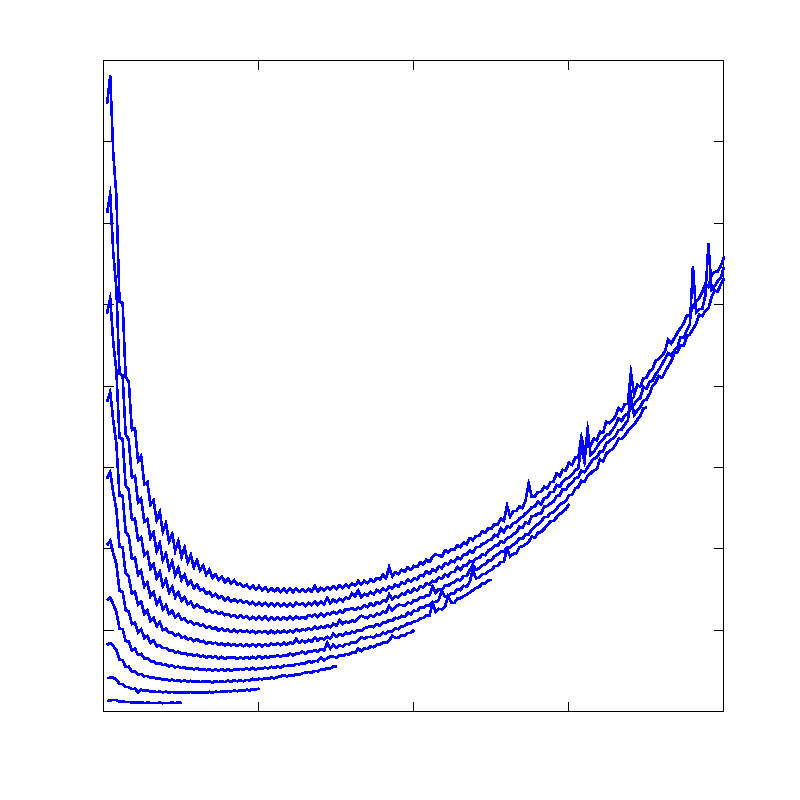
\includegraphics{images/performancePerNumBox}}%
    \gplfronttext
  \end{picture}%
\endgroup

                        \errorstopmode
                        \rule[-0.5cm]{0cm}{0cm}}
                \caption{Performance in function of the number of boxes for various strand lengths $N$ of ssDNA. The bottom curve corresponds to $N = 100$, each successively higher curve represents an additional 100 monomers, up to the top curve, where $N = 1000$.}
                \label{performancePerNumBox}
        \end{center}
\end{figure}


\begin{figure}[htb]
       \begin{center}
               \scalebox{0.9}{
                        \nonstopmode
                        % GNUPLOT: LaTeX picture with Postscript
\begingroup
  \makeatletter
  \providecommand\color[2][]{%
    \GenericError{(gnuplot) \space\space\space\@spaces}{%
      Package color not loaded in conjunction with
      terminal option `colourtext'%
    }{See the gnuplot documentation for explanation.%
    }{Either use 'blacktext' in gnuplot or load the package
      color.sty in LaTeX.}%
    \renewcommand\color[2][]{}%
  }%
  \providecommand\includegraphics[2][]{%
    \GenericError{(gnuplot) \space\space\space\@spaces}{%
      Package graphicx or graphics not loaded%
    }{See the gnuplot documentation for explanation.%
    }{The gnuplot epslatex terminal needs graphicx.sty or graphics.sty.}%
    \renewcommand\includegraphics[2][]{}%
  }%
  \providecommand\rotatebox[2]{#2}%
  \@ifundefined{ifGPcolor}{%
    \newif\ifGPcolor
    \GPcolortrue
  }{}%
  \@ifundefined{ifGPblacktext}{%
    \newif\ifGPblacktext
    \GPblacktexttrue
  }{}%
  % define a \g@addto@macro without @ in the name:
  \let\gplgaddtomacro\g@addto@macro
  % define empty templates for all commands taking text:
  \gdef\gplbacktext{}%
  \gdef\gplfronttext{}%
  \makeatother
  \ifGPblacktext
    % no textcolor at all
    \def\colorrgb#1{}%
    \def\colorgray#1{}%
  \else
    % gray or color?
    \ifGPcolor
      \def\colorrgb#1{\color[rgb]{#1}}%
      \def\colorgray#1{\color[gray]{#1}}%
      \expandafter\def\csname LTw\endcsname{\color{white}}%
      \expandafter\def\csname LTb\endcsname{\color{black}}%
      \expandafter\def\csname LTa\endcsname{\color{black}}%
      \expandafter\def\csname LT0\endcsname{\color[rgb]{1,0,0}}%
      \expandafter\def\csname LT1\endcsname{\color[rgb]{0,1,0}}%
      \expandafter\def\csname LT2\endcsname{\color[rgb]{0,0,1}}%
      \expandafter\def\csname LT3\endcsname{\color[rgb]{1,0,1}}%
      \expandafter\def\csname LT4\endcsname{\color[rgb]{0,1,1}}%
      \expandafter\def\csname LT5\endcsname{\color[rgb]{1,1,0}}%
      \expandafter\def\csname LT6\endcsname{\color[rgb]{0,0,0}}%
      \expandafter\def\csname LT7\endcsname{\color[rgb]{1,0.3,0}}%
      \expandafter\def\csname LT8\endcsname{\color[rgb]{0.5,0.5,0.5}}%
    \else
      % gray
      \def\colorrgb#1{\color{black}}%
      \def\colorgray#1{\color[gray]{#1}}%
      \expandafter\def\csname LTw\endcsname{\color{white}}%
      \expandafter\def\csname LTb\endcsname{\color{black}}%
      \expandafter\def\csname LTa\endcsname{\color{black}}%
      \expandafter\def\csname LT0\endcsname{\color{black}}%
      \expandafter\def\csname LT1\endcsname{\color{black}}%
      \expandafter\def\csname LT2\endcsname{\color{black}}%
      \expandafter\def\csname LT3\endcsname{\color{black}}%
      \expandafter\def\csname LT4\endcsname{\color{black}}%
      \expandafter\def\csname LT5\endcsname{\color{black}}%
      \expandafter\def\csname LT6\endcsname{\color{black}}%
      \expandafter\def\csname LT7\endcsname{\color{black}}%
      \expandafter\def\csname LT8\endcsname{\color{black}}%
    \fi
  \fi
  \setlength{\unitlength}{0.0500bp}%
  \begin{picture}(6720.00,4800.00)%
    \gplgaddtomacro\gplbacktext{%
      \colorrgb{0.00,0.00,0.00}%
      \put(741,528){\makebox(0,0)[r]{\strut{}10^{1}}}%
      \colorrgb{0.00,0.00,0.00}%
      \put(741,4439){\makebox(0,0)[r]{\strut{}10^{2}}}%
      \colorrgb{0.00,0.00,0.00}%
      \put(873,308){\makebox(0,0){\strut{}10^{2}}}%
      \colorrgb{0.00,0.00,0.00}%
      \put(6081,308){\makebox(0,0){\strut{}10^{3}}}%
      \colorrgb{0.00,0.00,0.00}%
      \put(-293,2483){\rotatebox{90}{\makebox(0,0){\strut{}\rule{0pt}{-1.5cm}Ideal number of boxes per dimension}}}%
      \colorrgb{0.00,0.00,0.00}%
      \put(3477,-22){\makebox(0,0){\strut{}Number of monomers}}%
    }%
    \gplgaddtomacro\gplfronttext{%
    }%
    \gplbacktext
    \put(0,0){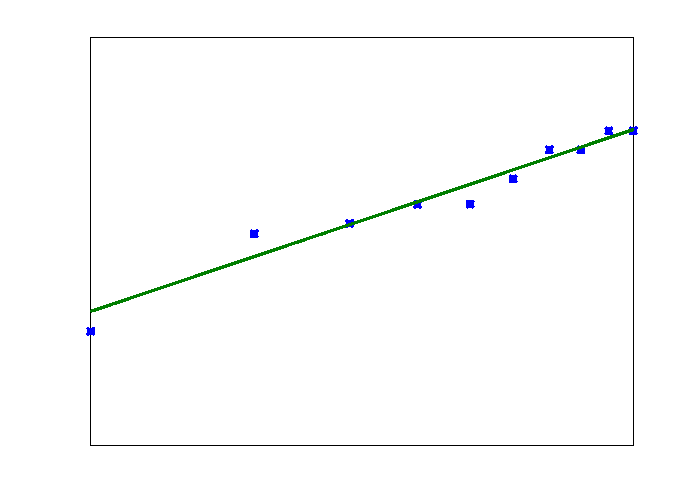
\includegraphics{images/numBoxExponentFit}}%
    \gplfronttext
  \end{picture}%
\endgroup

                        \errorstopmode
                        \rule[-0.5cm]{0cm}{0cm}}
                \caption{Ideal number of boxes per dimension in function of ssDNA strand length (logarithmic axes). The fitted curve has exponent $0.43 \pm 0.07$.}
                \label{numBoxExponentFit}
        \end{center}
\end{figure}


\begin{figure}[htb]
       \begin{center}
               \scalebox{0.9}{
                        \nonstopmode
                        % GNUPLOT: LaTeX picture with Postscript
\begingroup
  \makeatletter
  \providecommand\color[2][]{%
    \GenericError{(gnuplot) \space\space\space\@spaces}{%
      Package color not loaded in conjunction with
      terminal option `colourtext'%
    }{See the gnuplot documentation for explanation.%
    }{Either use 'blacktext' in gnuplot or load the package
      color.sty in LaTeX.}%
    \renewcommand\color[2][]{}%
  }%
  \providecommand\includegraphics[2][]{%
    \GenericError{(gnuplot) \space\space\space\@spaces}{%
      Package graphicx or graphics not loaded%
    }{See the gnuplot documentation for explanation.%
    }{The gnuplot epslatex terminal needs graphicx.sty or graphics.sty.}%
    \renewcommand\includegraphics[2][]{}%
  }%
  \providecommand\rotatebox[2]{#2}%
  \@ifundefined{ifGPcolor}{%
    \newif\ifGPcolor
    \GPcolortrue
  }{}%
  \@ifundefined{ifGPblacktext}{%
    \newif\ifGPblacktext
    \GPblacktexttrue
  }{}%
  % define a \g@addto@macro without @ in the name:
  \let\gplgaddtomacro\g@addto@macro
  % define empty templates for all commands taking text:
  \gdef\gplbacktext{}%
  \gdef\gplfronttext{}%
  \makeatother
  \ifGPblacktext
    % no textcolor at all
    \def\colorrgb#1{}%
    \def\colorgray#1{}%
  \else
    % gray or color?
    \ifGPcolor
      \def\colorrgb#1{\color[rgb]{#1}}%
      \def\colorgray#1{\color[gray]{#1}}%
      \expandafter\def\csname LTw\endcsname{\color{white}}%
      \expandafter\def\csname LTb\endcsname{\color{black}}%
      \expandafter\def\csname LTa\endcsname{\color{black}}%
      \expandafter\def\csname LT0\endcsname{\color[rgb]{1,0,0}}%
      \expandafter\def\csname LT1\endcsname{\color[rgb]{0,1,0}}%
      \expandafter\def\csname LT2\endcsname{\color[rgb]{0,0,1}}%
      \expandafter\def\csname LT3\endcsname{\color[rgb]{1,0,1}}%
      \expandafter\def\csname LT4\endcsname{\color[rgb]{0,1,1}}%
      \expandafter\def\csname LT5\endcsname{\color[rgb]{1,1,0}}%
      \expandafter\def\csname LT6\endcsname{\color[rgb]{0,0,0}}%
      \expandafter\def\csname LT7\endcsname{\color[rgb]{1,0.3,0}}%
      \expandafter\def\csname LT8\endcsname{\color[rgb]{0.5,0.5,0.5}}%
    \else
      % gray
      \def\colorrgb#1{\color{black}}%
      \def\colorgray#1{\color[gray]{#1}}%
      \expandafter\def\csname LTw\endcsname{\color{white}}%
      \expandafter\def\csname LTb\endcsname{\color{black}}%
      \expandafter\def\csname LTa\endcsname{\color{black}}%
      \expandafter\def\csname LT0\endcsname{\color{black}}%
      \expandafter\def\csname LT1\endcsname{\color{black}}%
      \expandafter\def\csname LT2\endcsname{\color{black}}%
      \expandafter\def\csname LT3\endcsname{\color{black}}%
      \expandafter\def\csname LT4\endcsname{\color{black}}%
      \expandafter\def\csname LT5\endcsname{\color{black}}%
      \expandafter\def\csname LT6\endcsname{\color{black}}%
      \expandafter\def\csname LT7\endcsname{\color{black}}%
      \expandafter\def\csname LT8\endcsname{\color{black}}%
    \fi
  \fi
  \setlength{\unitlength}{0.0500bp}%
  \begin{picture}(6720.00,4800.00)%
    \gplgaddtomacro\gplbacktext{%
      \colorrgb{0.00,0.00,0.00}%
      \put(741,528){\makebox(0,0)[r]{\strut{}0}}%
      \colorrgb{0.00,0.00,0.00}%
      \put(741,1017){\makebox(0,0)[r]{\strut{}500}}%
      \colorrgb{0.00,0.00,0.00}%
      \put(741,1506){\makebox(0,0)[r]{\strut{}1000}}%
      \colorrgb{0.00,0.00,0.00}%
      \put(741,1995){\makebox(0,0)[r]{\strut{}1500}}%
      \colorrgb{0.00,0.00,0.00}%
      \put(741,2484){\makebox(0,0)[r]{\strut{}2000}}%
      \colorrgb{0.00,0.00,0.00}%
      \put(741,2972){\makebox(0,0)[r]{\strut{}2500}}%
      \colorrgb{0.00,0.00,0.00}%
      \put(741,3461){\makebox(0,0)[r]{\strut{}3000}}%
      \colorrgb{0.00,0.00,0.00}%
      \put(741,3950){\makebox(0,0)[r]{\strut{}3500}}%
      \colorrgb{0.00,0.00,0.00}%
      \put(741,4439){\makebox(0,0)[r]{\strut{}4000}}%
      \colorrgb{0.00,0.00,0.00}%
      \put(873,308){\makebox(0,0){\strut{}0}}%
      \colorrgb{0.00,0.00,0.00}%
      \put(1915,308){\makebox(0,0){\strut{}200}}%
      \colorrgb{0.00,0.00,0.00}%
      \put(2956,308){\makebox(0,0){\strut{}400}}%
      \colorrgb{0.00,0.00,0.00}%
      \put(3998,308){\makebox(0,0){\strut{}600}}%
      \colorrgb{0.00,0.00,0.00}%
      \put(5039,308){\makebox(0,0){\strut{}800}}%
      \colorrgb{0.00,0.00,0.00}%
      \put(6081,308){\makebox(0,0){\strut{}1000}}%
      \colorrgb{0.00,0.00,0.00}%
      \put(-29,2483){\rotatebox{90}{\makebox(0,0){\strut{}\rule{0pt}{-1.5cm}CPU time in seconds per simulated nanosecond.}}}%
      \colorrgb{0.00,0.00,0.00}%
      \put(3477,-22){\makebox(0,0){\strut{}Number of monomers}}%
    }%
    \gplgaddtomacro\gplfronttext{%
    }%
    \gplbacktext
    \put(0,0){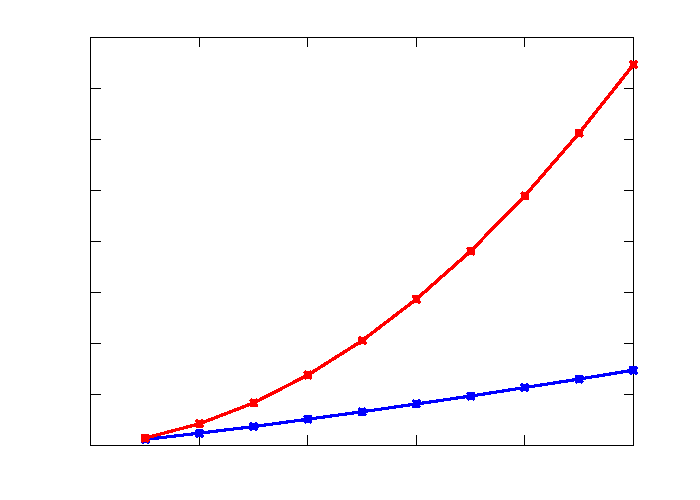
\includegraphics{images/spacePartVsNoSpacePart}}%
    \gplfronttext
  \end{picture}%
\endgroup

                        \errorstopmode
                        \rule[-0.5cm]{0cm}{0cm}}
                \caption{Performance of spatial partitioning with ideal number of boxes (blue curve) compared to naive quadratic pair search (corresponding to only a single box for the entire world, red curve).}
                \label{spacePartVsNoSpacePart}
        \end{center}
\end{figure}



The performance of our implementation for various strand lengths and number of boxes (per dimension) is shown in figure \ref{performancePerNumBox}. All performance simulations were run on an Intel Core2 Duo E8500 CPU. Note that there is an upper bound on the maximum number of boxes per dimension. Indeed, the length of a box cannot fall short of the potential truncation distance (in our case: $20$\,\Angstrom).

The ideal number of boxes for each strand length in figure \ref{performancePerNumBox} is plotted in figure \ref{numBoxExponentFit}. We find the relation $\bperdim \sim n^{0.43 \pm 0.07}$, where $\bperdim$ is the number of boxes in each dimension of the world (i.e, the total number of boxes $b$ is $(\bperdim)^3$).
This exponent $\bperdim$ is close to the value 1/3, implied by the theoretical argument above. The slightly higher value is possibly due to the fact that a world filled with a DNA strand is far less homogeneous than a world filled with a gas, or randomly bouncing particles.
Hence, there will be a significant amount of boxes that are completely empty, and vice versa a significant amount of boxes with a much higher than average number of particles (sites).
Caching in modern CPUs may also play a role, in the sense that large numbers of monomers and boxes imply that the entire working set does not fit in the fastest cache levels on the CPU, potentially giving a bias to smaller boxes (though we can't immediately see a reason for this).

Lastly, the performance scaling with the ideal number of boxes is compared to the scaling without space partitioning in figure \ref{spacePartVsNoSpacePart}. The quadratic trend of the naive method is clearly worse than the linear scaling when space partitioning is enabled.

